% DO NOT COMPILE THIS FILE DIRECTLY!
% This is included by the other .tex files.

\begin{frame}[t,plain]
\titlepage
\end{frame}

\begin{frame}
    \frametitle{Who am I}
    \begin{minipage}{0.6\textwidth}
        \begin{itemize}
            \item \faGithub : chrisr3d \\
            \item \faMastodon : @chrisr3d@infosec.exchange
            \item \faTwitter : chrisred\_68
            \item []
            \item Interoperability Wizard @ CIRCL
            \item MISP core development team
            \item STIX SC co-chair
            \item []
            \item \faCat \vspace{1em} \& \faCamera \vspace{1em} enthusiast
        \end{itemize}
    \end{minipage}%
    \begin{minipage}{0.4\textwidth}
        
\includegraphics[scale=0.1]{images/profile_picture.jpg}
    \end{minipage}
\end{frame}

\begin{frame}
    \frametitle{Summary}
    \begin{itemize}
        \item From an ocean of unknown errors...\linebreak $\Rightarrow$ the difficulty to parse STIX content
        \item ... To a more \& more accurate support\linebreak $\Rightarrow$ \emph{misp-stix} - The Holy Grail for MISP \& STIX
        \item ... And even further\linebreak $\Rightarrow$ Evolution \& improvement perspectives
        \item The magic word: \emph{interoperability}
        \item Demo (?)
    \end{itemize}
\end{frame}

\begin{frame}
    \frametitle{STIX - Quick recap}
    \begin{minipage}{0.5\textwidth}
        \centering
        
\includegraphics[scale=0.5]{images/LOGO_STIX.pdf}
    \end{minipage}%
    \begin{minipage}{0.5\textwidth}
        \centering
        
\includegraphics[scale=0.45]{images/LOGO_TAXII.pdf}
    \end{minipage}
    \vspace{1em}
    \begin{itemize}
        \item \textbf{S}tructured \textbf{T}hreat \textbf{I}ntelligence E\textbf{x}pression
        \begin{itemize}
            \item Focused on \textbf{Threat Intelligence} exchange
            \item 2 major versions with different formats
            \begin{itemize}
                \item 1.x - \emph{mostly} XML
                \item 2.x - JSON
            \end{itemize}
        \end{itemize}
        \item \textbf{T}rusted \textbf{A}utomated E\textbf{x}change of \textbf{I}ntelligence \textbf{I}nformation
        \begin{itemize}
            \item Exchange Protocol
            \item Specifically designed to support the exchange of \textbf{CTI} represented in STIX
        \end{itemize}
    \end{itemize}
\end{frame}

\begin{frame}
    \frametitle{STIX 1.x - a tough beast to handle}
    \centering
    
\includegraphics[scale=0.54]{images/xml.jpg}
\end{frame}

\begin{frame}
    \frametitle{STIX 1.x - a tough beast to handle}
    \begin{itemize}
        \item Excessive complexity in certain advanced XML constructs
        \begin{itemize}
            \item Difficult to implement \& parse
        \end{itemize}
        \item A plethora of different objects
        \begin{itemize}
            \item Only a common subset of capabilities widely used
            \item Many others poorly understood and in many cases never used 
        \end{itemize}
        \item Multiple ways to represent an information
        \begin{itemize}
            \item Challenging for interoperability
        \end{itemize}
        \item A majority of optional properties
        \begin{itemize}
            \item Parsing challenges for consumers of STIX 1 content
        \end{itemize}
    \end{itemize}
\end{frame}

\begin{frame}
    \frametitle{STIX 2.x - an improvement}
    \centering
    
\includegraphics[scale=0.45]{images/json.jpg}
\end{frame}

\begin{frame}
    \frametitle{STIX 2.x - an improvement}
    \begin{itemize}
        \item Lightweight \& flattened representation of the objects
        \item More required properties
        \begin{itemize}
            \item Easier to parse
        \end{itemize}
        \item Extension definitions
        \begin{itemize}
            \item More flexibility
        \end{itemize}
        \item []
        \item []\hspace{1em} \linebreak \hspace{1em}  \linebreak \hspace{1em}
        \item []\hspace{1em} \linebreak \hspace{1em}  \linebreak \hspace{1em}
    \end{itemize}
\end{frame}

\begin{frame}
    \frametitle{STIX 2.x - the (still not perfect) improvement}
    \begin{itemize}
        \item Lightweight \& flattened representation of the objects
        \item More required properties
        \begin{itemize}
            \item Easier to parse
        \end{itemize}
        \item Extension definitions
        \begin{itemize}
            \item More flexibility
        \end{itemize}
        \item Number of objects reduced to a set of well-understood features
        \linebreak \faPlusCircle \hspace{0.3em} Clearer for everyone
        \linebreak \faMinusCircle \hspace{0.3em} Some definitions lost in the process
        \item Introduction of patterns within Indicator objects
        \linebreak \faPlusCircle \hspace{0.3em} Ability to use different patterning languages (STIX 2.1)
        \linebreak \faMinusCircle \hspace{0.3em} Observations and Indicators need distinct parsing
        \item Still multiple ways to represent the same data
    \end{itemize}
\end{frame}

\begin{frame}
    \frametitle{The reality about STIX parsing}
    \centering
    
\includegraphics[scale=0.45]{images/hell.png}
\end{frame}

\begin{frame}
    \frametitle{Struggling with various STIX pattern creation designs}
    \begin{itemize}
        \item Handling the multiple ways of reprensenting the \emph{same} concept
        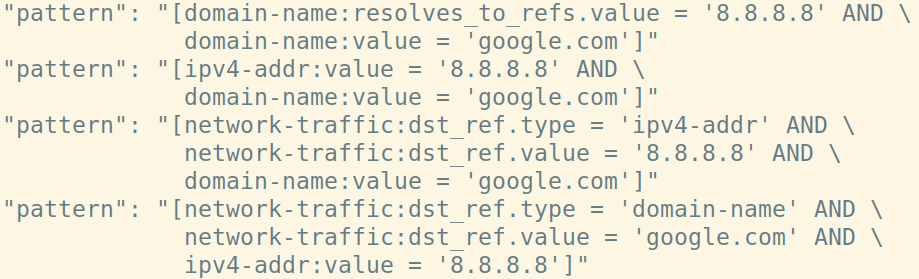
\includegraphics[scale=0.3]{images/pattern1.png}
        \item Understanding the meaning of data
        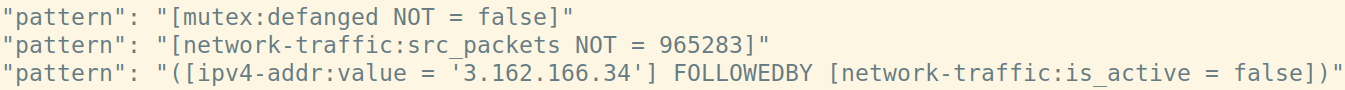
\includegraphics[scale=0.3]{images/pattern2.png}
    \end{itemize}
\end{frame}

\begin{frame}
    \frametitle{Struggling with various STIX pattern creation designs}
    \begin{minipage}{0.5\textwidth}
        \centering
        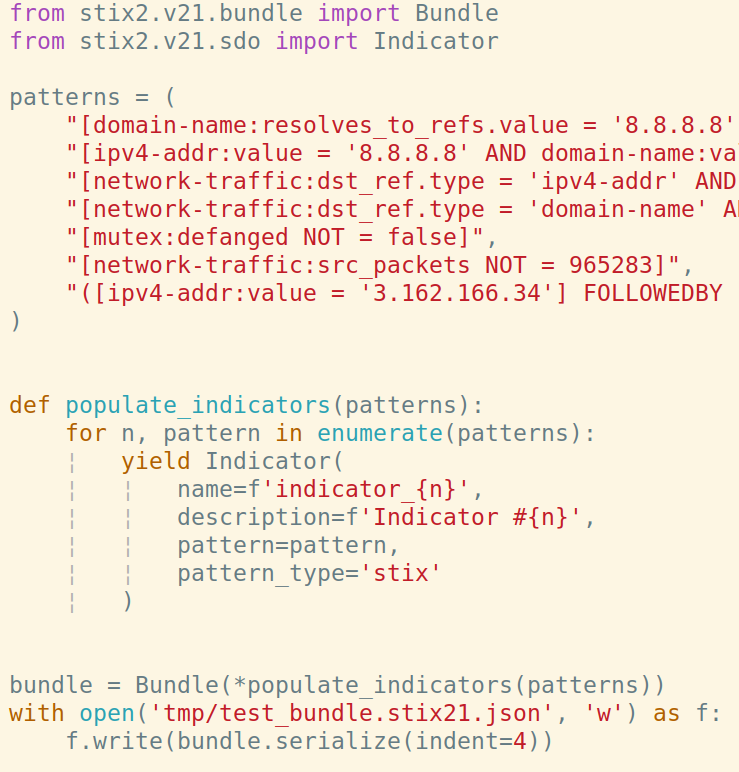
\includegraphics[scale=0.25]{images/generate_indicators.png}
    \end{minipage}%
    \begin{minipage}{0.5\textwidth}
        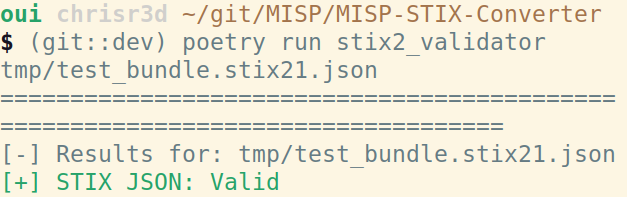
\includegraphics[scale=0.3]{images/stix2_validator.png}
    \end{minipage}
\end{frame}

\begin{frame}
    \frametitle{The constant validation issues}
    \begin{minipage}{0.7\textwidth}
        \begin{itemize}
            \item We want to \textbf{keep UUIDs} for referencing
            \item []
            \item Not everyone validates their content properly
            \pause
            \item []
            \item Issues with UUIDs validation
            \begin{itemize}
                \item Unable to load content
            \end{itemize}
        \end{itemize}
    \end{minipage}%
    \begin{minipage}{0.3\textwidth}
        
\includegraphics[scale=0.25]{images/two_buttons_dilemna.jpg}
    \end{minipage}
\end{frame}

\begin{frame}
    \frametitle{An easy fix - Making the UUIDs validation more flexible}
    \begin{minipage}{0.7\textwidth}
        \begin{itemize}
            \item STIX 2 python library fork\footnotemark[1]
            \begin{itemize}
                \item No change on the content validation
                \item Differs only on the UUIDs validation
            \end{itemize}
            $\Rightarrow$ Same UUIDs requirements on MISP \& STIX
            \item[]
            \item Handling the "\emph{worst}" UUIDs
            \begin{itemize}
                \item Generating a v5 UUID to be used as new identifier
                \item Keeping a reference to the initial UUID
            \end{itemize}
        \end{itemize}
    \end{minipage}%
    \begin{minipage}{0.3\textwidth}
        
\includegraphics[scale=0.25]{images/two_buttons_solution.jpg}
    \end{minipage}
    \footnotetext[1]{\url{https://github.com/MISP/cti-python-stix2}\hspace{1em}-\hspace{1em}\url{https://pypi.org/project/misp-lib-stix2/}}
\end{frame}

\begin{frame}
    \frametitle{\emph{misp-stix} - The Holy Grail for MISP \& STIX interactions}
    \centering
    
\includegraphics[scale=0.3]{images/solution.png}\footnote{\url{https://github.com/MISP/misp-stix}\hspace{1em}-\hspace{1em}\url{https://pypi.org/project/misp-stix/}}
    \setcounter{footnote}{0}
\end{frame}

\begin{frame}
    \frametitle{\emph{misp-stix} - The Holy Grail for MISP \& STIX interactions}
    \begin{minipage}{0.7\textwidth}
        \begin{itemize}
            \item Used in MISP
            \begin{itemize}
                \item Conversion only
            \end{itemize}
            \item Can be used as a \textbf{stand-alone} tool \footnotemark[1]
            \begin{itemize}
                \item Converting input file(s), saving results in output file(s)
            \end{itemize}
            \item Enabling automation with python code
            \begin{itemize}
                \item Handles both conversion and input(s)/output(s)
                \item Supports all the available input formats
                \begin{itemize}
                    \item file names, JSON, PyMISP, STIX Packages or Bundles
                \end{itemize}
            \end{itemize}
        \item []
        \item A complete mapping documentation\footnotemark[2]
        \end{itemize}
    \end{minipage}%
    \begin{minipage}{0.3\textwidth}
        \centering
        
\includegraphics[scale=0.2]{images/LOGO_MISP_STIX.png}
    \end{minipage}
    \footnotetext[1]{i.e Command line}
    \footnotetext[2]{\url{https://github.com/MISP/misp-stix/tree/main/documentation}}
\end{frame}
